\documentclass{beamer}
\usepackage{amsmath, amsfonts, amssymb, amsthm}
\usepackage{graphicx, caption, hyperref, url, cite}
\usepackage[UTF8, noindent]{ctexcap}

\usetheme{Boadilla}

\title{汇报0518}
% \subtitle{项目三:基于大规模预训练模型的生成式知识问答}
\institute{项目三}
\author{朱睿涵 \and 李宸亦}
\date{\today}

\setbeamertemplate{bibliography item}[text]

\begin{document}

\frame{\titlepage} % 标题页

\AtBeginSection{
    \begin{frame}
        \frametitle{目录}

        \tableofcontents[currentsection]
    \end{frame}
}

\section{pytorch实现baseline}
\begin{frame}
    \frametitle{实验所用数据}
    所使用预训练模型:BERT-wwm-ext, Chinese

    训练数据集:WebQA和SougouQA

    测试数据集:SougouQA

    google bert模型
\end{frame}

\begin{frame}
    \frametitle{实验过程}
    \begin{enumerate}
        \item 划分数据集, 生成数据
        \item 调用unilm进行训练
        \item 进行阅读理解任务
        \item 使用SougouQA数据集测试模型
        \item 汇总最终结果
    \end{enumerate}
\end{frame}



\begin{frame}
    \frametitle{结果}
    苏剑林模型的结果:Accuracy=0.7259005836184343,F1=0.813860036706151,Final=0.7698803101622926

    本次实验结果:
    \begin{figure}
        \centering
        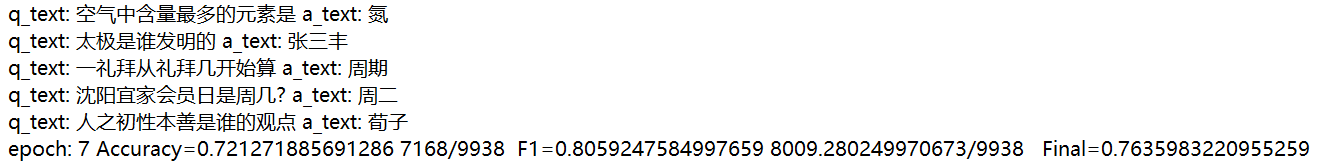
\includegraphics[width=0.95\textwidth]{./fig/result.png}
    \end{figure}

\end{frame}


\section{实验中遇到的问题}
\begin{frame}
    \frametitle{实验中遇到的问题}
    \begin{itemize}
        \item 调研论文寻找困难
        \item 不清楚预训练微调过程
        \item 计算资源不稳定
    \end{itemize}


\end{frame}

\begin{frame}{References}

    \nocite{*}
    \bibliographystyle{unsrt}
    \bibliography{reference.bib}

\end{frame}
\end{document}